\chapter{Technologien und Werkzeuge}
\label{cha:technologie_werkzeuge}
Die verwendeten Technologien und Werkzeuge sind für diese Arbeit wesentlich, um die Implementierung nachvollziehen zu können. Die Entwicklungsplattform .NET spielt dabei für das entwickelte Framework eine entscheidende Rolle, wie bereits in Unterabschnitt \ref{subsec:patterns} bei den beschriebenen Patterns erwähnt. In diesem Kapitel werden daher einige zentrale Konzepte vorgestellt.

\section{Visual Studio}
\label{sec:visual_studio}

Für C\# (Unterabschnitt \ref{subsec:csharp}) existieren mehrere Entwicklungsumgebungen, wie zum Beispiel JetBrains Rider oder Visual Studio. Da die in dieser Arbeit erstellte Software in einem produktiven Umfeld eingesetzt werden soll, in dem Visual Studio verwendet wird, wurde für die Entwicklung ebenfalls Visual Studio 2022 eingesetzt. 

Visual Studio ist eine komplexe Integrated Development Environment (IDE) von Microsoft und beinhaltet Funktionalitäten zum Erstellen, Debuggen, Testen und weitere nützliche Features, wie in der offiziellen Dokumentation beschrieben \cite{MicrosoftVisualStudioIDE2022}.

\section{.NET}
\label{sec:dotnet}
Für die Umsetzung der Implementierung in Kapitel \ref{cha:implementierung} wird die von Microsoft bereitgestellte Laufzeitumgebung und Entwicklungsplattform .NET \cite{dotnet} in der Version 8 \footnote{Microsoft veröffentlicht alle zwei Jahre eine Long-Term-Support-Version (LTS) von .NET. Version 8 wurde im November 2024 bereitgestellt und bietet langfristigen Support. Darüber hinaus erscheint jährlich im November eine neue .NET-Version.} verwendet. Diese Version enthält bereits die beiden UI-Frameworks WPF (siehe Unterabschnitt \ref{subsec:WPF}) und Windows Forms (siehe Unterabschnitt \ref{subsec:Winforms}), die ausschließlich unter Windows-Betriebssystemen eingesetzt werden können. Die für diese Arbeit relevanten Konzepte und Funktionen von .NET werden in diesem Kapitel näher erläutert.

\subsection{C\#}
\label{subsec:csharp}
Für die .NET-Plattform stehen mehrere Programmiersprachen zur Verfügung, darunter C\#, F\# und VB.NET. Für die Entwicklung des Frameworks wird C\# verwendet. Diese Sprache gilt laut Microsoft \cite{microsoft-tour-of-csharp} als die beliebteste Sprache innerhalb des .NET-Ökosystems und basiert auf dem objektorientierten Paradigma. Darüber hinaus integriert C\# Konzepte aus weiteren Programmierparadigmen, wie der funktionalen Programmierung. Ein Beispiel für die funktionale Programmierung ist Language Integrated Query (LINQ), das typisierte Abfragen in einer SQL-ähnlichen Syntax direkt im Code ermöglicht.

\subsubsection{Übersetzung und Ausführung}
C\# wird, wie auch andere Sprachen desselben Ökosystems, zunächst in IL (Intermediate Language) übersetzt. Dieser IL-Code wird anschließend durch die Common Language Runtime (CLR) \cite{microsoft-clr-overview} in nativen Maschinencode umgewandelt. Standardmäßig erfolgt diese Übersetzung in .NET über den Just-in-Time-Compiler (JIT). Es existieren jedoch auch Varianten, bei denen Anwendungen bereits teilweise oder vollständig vor der Ausführung in nativen Code kompiliert werden (Ahead-of-Time-Kompilierung \cite{microsoft-native-aot}).

Für die Ausführung von .NET-Programmen wird somit die CLR benötigt, die Bestandteil der .NET Runtime Environment bzw. des .NET SDK ist. Die Assemblies (siehe Unterabschnitt \ref{subsec:assemblies}) werden üblicherweise als \texttt{.dll}- oder \texttt{.exe}-Dateien abgelegt, unterscheiden sich inhaltlich jedoch von C++ Programmen, die nativ kompiliert werden.

\subsection{Nullable Reference Types}
Der bekannte Informatiker Tony Hoare bezeichnete die Einführung von \texttt{null} als seinen größten Fehler, da die dadurch verursachten Probleme enorm seien \cite{hoare_null_video}. Dieses Problem lässt sich bis zu einem gewissen Grad durch die sogenannten Nullable Reference Types \cite{microsoft-nullable-references} lösen. Der Compiler prüft hierbei, ob eine Variable den Wert \texttt{null} annehmen kann und falls dies der Fall ist, muss der Code explizit eine entsprechende Überprüfung vorsehen. Aufgrund der damit verbundenen Reduzierung von NullReferenceException-Fehlern wird dieses Konzept auch in dieser Arbeit verwendet. Entscheidend ist jedoch, dass die durch den Compiler entstehenden Warnings auf Errors umgestellt werden, um die Abdeckung aller entstandenen Nullszenarien zu garantieren.

\subsection{Assemblies}
\label{subsec:assemblies}
Die Erzeugnisse des Kompilierungsprozesses werden in .NET als Assemblies \cite{msdn_assembly_manifest} bezeichnet. Für Assemblies existieren zwei Dateitypen: \texttt{.dll} und \texttt{.exe}. Assemblies des Typs \texttt{.exe} sind ausführbare Dateien, während Assemblies des Typs \texttt{.dll} Klassenbibliotheken bzw. andere Programmteile darstellen, die wiederverwendet werden können.

\subsubsection{Erzeugung von Assemblies}
Abbildung \ref{fig:assemblies_dotnet} zeigt, wie eine Assembly aus mehreren Quelldateien erzeugt wird. Dabei wird das MSBuild-File verwendet, um dem Compiler die erforderlichen Schritte mitzuteilen. Der Compiler erzeugt anschließend aus den Ressourcen und den C\#-Dateien (siehe Unterabschnitt \ref{subsec:csharp}) eine Assembly. Dabei werden die Ressourcen, Metadaten und der IL-Code in die resultierende Datei eingebettet.

\begin{figure}[H]
    \centering
    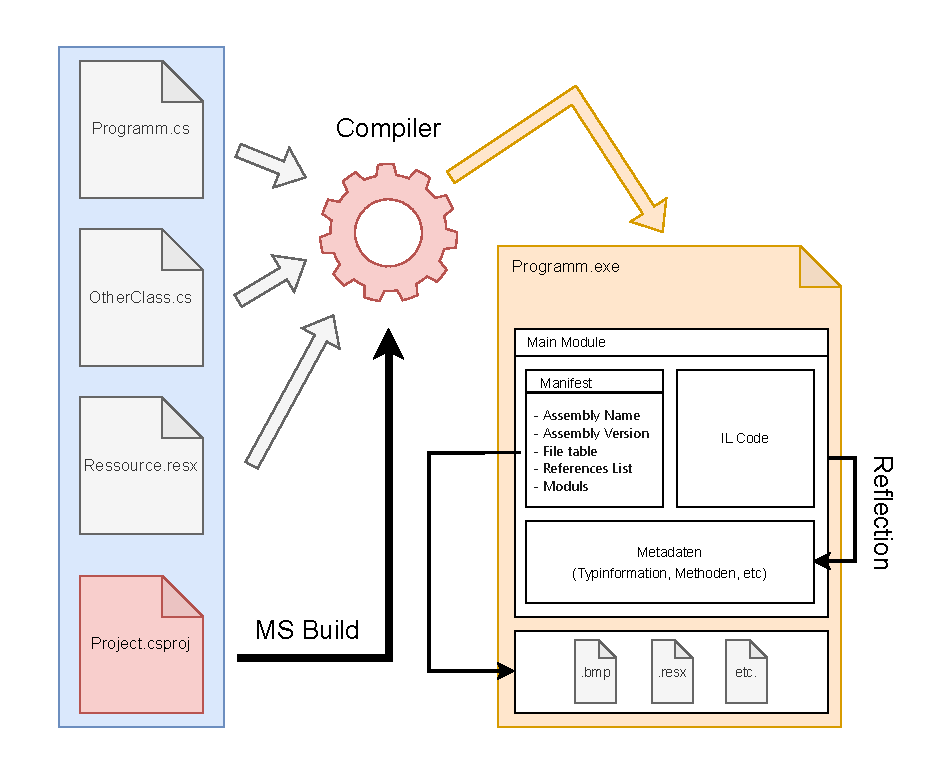
\includegraphics[width=0.9\textwidth]{3_Assemblies_Dotnet}
    \caption{Assemblies Aufbau und Generierung}
    \label{fig:assemblies_dotnet}
\end{figure}

\subsubsection{Aufbau einer Assembly}
Eine Assembly besteht, wie in Abbildung \ref{fig:assemblies_dotnet} dargestellt, aus mehreren Modulen. Diese sogenannten Module enthalten IL-Code und Metadaten, wobei das Hauptmodul zusätzlich ein Manifest beinhaltet.  
Der IL-Code (Intermediate Language) stellt eine Zwischensprache zwischen Maschinencode und der Programmiersprache dar und enthält die Anweisungen, die letztlich ausgeführt werden.  
Die Metadaten enthalten Informationen über Methodensignaturen, Typen und weitere Strukturdaten. Diese Metainformationen bilden zusammen mit Reflection (siehe Unterabschnitt \ref{subsec:reflection}) einen wichtigen Bestandteil der Laufzeitumgebung. Weiters enthält das erwähnte Manifest folgende Informationen:

\begin{itemize}
    \item Assembly Name
    \item Assembly Version: Wesentlich, da Assemblies die kleinstmögliche Einheit der Versionierung darstellen. Dies ermöglicht beispielsweise die gleichzeitige Verwendung verschiedener Versionen einer Klassenbibliothek in einem Projekt, ohne dass Assemblies überschrieben werden.
    \item File Table: Listet die eingebetteten Ressourcen auf.
    \item References List: Listet die Abhängigkeiten zu anderen Assemblies auf.
    \item Modules: Gibt an, welche Module in einer Assembly enthalten sind. Im Standardfall, wie in Abbildung \ref{fig:assemblies_dotnet} dargestellt, existiert nur ein Modul.
\end{itemize}

Da Assemblies im PE-Format (Portable Executable) \cite{MicrosoftLearn_PEFormat} gespeichert werden, enthalten sie zusätzlich alle für dieses Format erforderlichen Informationen.

\subsection{Reflection}
\label{subsec:reflection}
In Abbildung \ref{fig:assemblies_dotnet} zeigt ein Pfeil vom IL-Code zu den Metadaten. Dies verdeutlicht, dass in C\# (siehe Unterabschnitt \ref{subsec:csharp}) ein Mechanismus namens \textit{Reflection} \cite{MicrosoftLearn_Reflection} existiert, der es ermöglicht, Metainformationen über Typen, Methoden oder Attribute zur Laufzeit abzufragen und zu manipulieren. 

Reflection basiert auf speziellen IL-Instruktionen, die über die .NET-API auch in C\# zugänglich sind. Dadurch kann ein Programm beispielsweise alle Eigenschaften eines bestimmten Typs ermitteln und deren Werte dynamisch auslesen oder ändern. 

Reflection ist ein sehr mächtiges Werkzeug, bringt jedoch Leistungseinbußen mit sich. Der Zugriff auf Werte oder Typinformationen über Reflection ist deutlich langsamer als ein zur Compilezeit generierter Zugriff. Das liegt daran, dass die zugrunde liegenden Type- und MemberInfo-Objekte beim ersten Zugriff aus den Assembly-Metadaten erzeugt und anschließend zwischengespeichert werden müssen. Jeder weitere Zugriff erfolgt indirekt über mehrere Objekte, wodurch zusätzliche Zwischenschritte, ähnlich wie bei einer virtuellen Methodentabelle, notwendig werden. Die Auswirkungen von Reflection auf die Laufzeit werden in einem Artikel auf MSDN näher beschrieben \cite{Pobar2005_PerformancePitfalls}.


\subsection{Asynchrone Programmierung}
\label{subsec:async}
Für trackingbasierte Prozesse ist es wichtig, dass diese die Usability des bestehenden Systems nicht beeinträchtigen. Würden Tracking-Abläufe synchron mit der Benutzeroberfläche ausgeführt werden, könnte die UI währenddessen nicht auf Benutzereingaben reagieren. Daher spielt die asynchrone Programmierung eine entscheidende Rolle in dieser Arbeit.

\subsection{Grundlegende Funktionsweise}
Um Aufgaben nebenläufig ausführen zu können, bietet .NET (Abschnitt \ref{sec:dotnet}) die Möglichkeit, Threads zu verwenden. Threads sind leichtgewichtige Prozesse, die denselben Heap teilen, jedoch jeweils über einen eigenen Stack verfügen. Sie sind, abhängig vom Betriebssystem, ein grundlegender Bestandteil des Systems. Threads können zur Laufzeit erzeugt werden und führen dann Methoden wie im Programm \ref{prog:thread_based_programming} gezeigt aus. Nach Abschluss der Methode beendet sich der Thread und die Ressourcen werden vom Betriebssystem freigegeben. Threads sind ein zentraler Bestandteil von .NET und werden in einem Artikel von Microsoft \cite{Microsoft_ThreadsAndThreading} näher beschrieben.

\begin{program}[H]
\begin{CsCode}
Thread workerThread = new Thread(() => Console.WriteLine("Arbeit beendet"));

Console.WriteLine("Starte Arbeit");
workerThread.Start();
\end{CsCode}
\caption{Erzeugen eines Threads}
\label{prog:thread_based_programming}
\end{program}

Da das Erzeugen von Threads Systemressourcen kostet, stellt C\# (Unterabschnitt \ref{subsec:csharp}) die ThreadPool-Klasse bereit. Diese erzeugt eine feste Anzahl an Threads, die wiederverwendet werden. Aufgaben werden als Arbeitspakete an diese Threads delegiert. Alle in C\# vorgestellten Konzepte der asynchronen Programmierung nutzen diesen Pool standardmäßig.

\subsubsection{Konzepte der asynchronen Programmierung in C\#}
In C\# (siehe Unterabschnitt \ref{subsec:csharp}) existieren mehrere Konzepte, um Abläufe verzahnt (auf einem einzelnen Kern) oder parallel (auf mehreren Kernen) auszuführen, wie im Buch \cite{sarcar2004design} beschrieben. Zu diesen Konzepten zählen:

\begin{itemize}
    \item \textbf{Asynchronous Programming Model:} Umsetzung über Delegate.BeginInvoke und Delegate.EndInvoke.
    \item \textbf{Event-based Asynchronous Pattern:} Ein Thread führt eine Aufgabe aus und informiert einen Observer über deren Abschluss.
    \item \textbf{Task-based Asynchronous Pattern:} Ein Task ist eine Einheit, die eine bestimmte Aufgabe ausführt und Informationen über deren Status enthält.
\end{itemize}

In dieser Arbeit wird das Task-based Asynchronous Pattern verwendet, da es die Nutzung von async und await ermöglicht.

\subsubsection{Task-based Asynchronous Pattern}
Ein Task \cite{Microsoft_TaskClass} repräsentiert eine definierte Aufgabe. Diese wird standardmäßig auf einem Thread aus dem ThreadPool ausgeführt. Ein Task ermöglicht es, auf seine Fertigstellung zu warten oder nach Abschluss eine Fortsetzung auszuführen. Diese Fortsetzung kann im gleichen Synchronization Context oder in einem anderen Kontext erfolgen, um Deadlocks zu vermeiden. Ein Deadlock kann beispielsweise auftreten, wenn auf einen Task blockierend in einem Thread gewartet wird, der jedoch für die Fortsetzung des Tasks erforderlich ist. Ein Beispiel für asynchronen Code wird in Programm \ref{prog:aync_task_based} gezeigt.

\begin{program}[H]
\begin{CsCode}
Console.WriteLine("Arbeit starten");

Task resultTask = Task.Run(async () =>
{
    for (int i = 0; i < 100; i++)
        await Task.Delay(100);

    Console.WriteLine("Arbeit fertiggestellt");
});

Console.WriteLine("Ohne Arbeit fortsetzen");

await resultTask; // alternativ: .Wait() für synchrones Warten
Console.WriteLine("Arbeit sicher fertig");
\end{CsCode}
\caption{Asynchrone Programmierung mit Tasks}
\label{prog:aync_task_based}
\end{program}

\section{UI-Frameworks}
\label{sec:ui_frameworks}
In diesem Abschnitt werden die UI-Frameworks aus der .NET-Umgebung (siehe Abschnitt \ref{sec:dotnet}) vorgestellt, in die das Aktivitäts-Tracking-Framework integriert werden kann. Für diese Frameworks ist insbesondere das Event-System von Bedeutung, da es ein Tracking durch die Verfolgung von Benutzeraktionen, wie z.B. Button-Klicks, ermöglicht.

\subsection{WPF}
\label{subsec:WPF}
Windows Presentation Foundation \cite{microsoft_wpf_overview} ist ein Framework zur Entwicklung von Windows-Desktop-Applikationen. Es baut auf dem in Abschnitt \ref{fig:mvvm_pattern} erläuterten MVVM-Pattern auf und verwendet für das Erstellen der Ansichten XAML, einen XML-Dialekt. 

Um die UI-Elemente anzusteuern, gibt es eine Code-Behind-Datei, welche eine Partial-Klasse zu der aus dem XAML generierten Klasse darstellt. Dort können Events behandelt oder anderer view-spezifischer Code ausgeführt werden. Dies wird im Buch \cite{james2015pro} näher erläutert und an Beispielen dargestellt.

\subsubsection{Event-System}
Events stellen die Basis für den Zugriff auf das Verhalten in einer Ansicht dar. WPF bietet hierzu \emph{Routed Events} \cite{microsoft_wpf_routed_events_overview} an. Routed Events sind Events, die im Elementbaum wandern können und die entsprechenden registrierten Handler im Baum informieren. WPF bietet hierfür folgende drei Modelle für das Wandern durch den Baum an:

\begin{itemize}
    \item \textbf{Bubbling}: Das Event wandert von der Source zum Wurzelelement (Window)
    \item \textbf{Tunneling}: Das Event wandert von der Wurzel zur Source
    \item \textbf{Direct}: Nur Handler auf der Source werden über das Ereignis informiert
\end{itemize}

\begin{figure}[H]
    \centering
    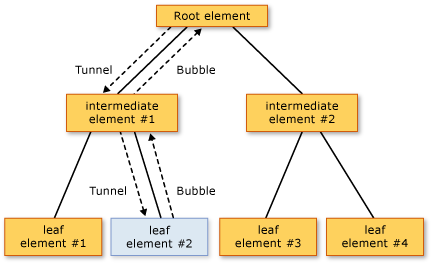
\includegraphics[width=0.6\textwidth]{3_Routed_Events}
    \caption{Reihenfolge Ereignisverarbeitung. Quelle: \cite{microsoft_wpf_routed_events_overview}}
    \label{fig:routed_events}
\end{figure}

In der Abbildung \ref{fig:routed_events} werden Tunneling und Bubbling durch Pfeile im Elementbaum dargestellt. Dabei soll unter anderem gezeigt werden, dass Preview-Events das Tunneling-Verfahren verwenden und erst anschließend das eigentliche Event über Bubbling propagiert wird.

\subsection{Windows Forms}
\label{subsec:Winforms}
Windows Forms \cite{microsoft_winforms_overview} ist die Vorgängertechnologie von WPF (siehe Unterabschnitt \ref{subsec:WPF}) und besteht ebenfalls aus einer Designer-Datei und einer Code-Behind-Datei. Die Designer-Datei enthält dabei direkt Code, der den Aufbau des Steuerelementbaums beschreibt, während die Code-Behind-Datei die Anwendungslogik implementiert. Windows Forms basiert nicht explizit auf einem Design-Pattern wie MVVM (siehe Unterabschnitt \ref{subsec:mvvm}). Im zu integrierenden System wird jedoch das MVP-Pattern verwendet (siehe Unterabschnitt \ref{subsec:mvp}). Dadurch befindet sich in der Code-Behind-Datei nur noch die für die View notwendige Anzeigelogik.

\subsubsection{Event-System}
Events in Windows Forms \cite{microsoft_winforms_events_overview} sind grundsätzlich nicht routed, sondern werden nur von den am jeweiligen Steuerelement registrierten Event-Handlern verarbeitet. Es gibt jedoch Ausnahmen bei Steuerelementen, die keinen eigenen Fenster-Handle besitzen und daher keine Events direkt empfangen können. In diesen Fällen übernimmt das übergeordnete Steuerelement (Parent) die Ereignisverarbeitung und leitet das Event gegebenenfalls weiter. Solche Events können somit sowohl vom Parent- als auch vom Child-Element behandelt werden. Das Verhalten hängt dabei häufig von Einstellungen wie KeyPreview \cite{microsoft_form_keypreview} ab und muss entsprechend berücksichtigt werden.




